\documentclass{standalone}
\usepackage{tikz}
\usepackage{verbatim}
\begin{document}
\pagestyle{empty}
  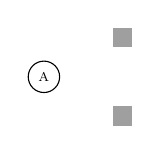
\begin{tikzpicture}
    \node[draw,circle,scale=2/3] (a) at (+0, 0) {\scriptsize A};
    \node[draw,circle, scale=0.3] (g) at (+1, 0.5) {};
    \node[draw,circle, scale=0.3] (b) at (+1, -0.5) {};
    \node[draw,rectangle,fill,gray!75] (p) at (+1, 0.5) {};
    \node[draw,rectangle,fill,gray!75] (n) at (+1, -0.5) {};
  \end{tikzpicture}
\end{document}